\documentclass[9pt]{beamer}

% there was some issue with the fonts. using exactly what normal latex does is pretty good enough
\usefonttheme{serif}
\usepackage[T1]{fontenc}
\usepackage{lmodern}

% theme
\usetheme{Boadilla}
\usecolortheme{crane}
\setbeamertemplate{navigation symbols}{}

% danish added below line to be able to add references and citations and links in the document
\usepackage{hyperref}

% to be able to verbatim
\usepackage{listings}

% to be able to add references
\usepackage{biblatex}
\addbibresource{references.bib}

% \usepackage{annotate-equations}
\usepackage{pgfplots}
\pgfplotsset{compat=1.18}
\usepackage{tikz}
\usetikzlibrary{arrows.meta,math,positioning,fit}
\tikzset{
    declare function={
        objective(\x,\y) = 0.5*(\x-1)^2 + (\y-2)^2;
    }
}

\usepackage{threeparttable}

\title[MSc. AI Thesis]{Causal Discovery in the presence of Latent Confounders}
\subtitle{A Stochastic Optimization Approach}
\author[Danish Mohammad]{Danish Shakeel Mohammad}
\date{\today}

\institute[QMUL]{Queen Mary, University of London}

\begin{document}
    \maketitle
    \begin{frame}{Introduction}
        \uncover<1-6>{
        \begin{block}{}
            \centering
            Causal Discovery is the automated extraction of cause and effect relationships from data.
        \end{block}
    }

        \begin{columns}[T, onlytextwidth]
            \begin{column}{0.60\textwidth}
                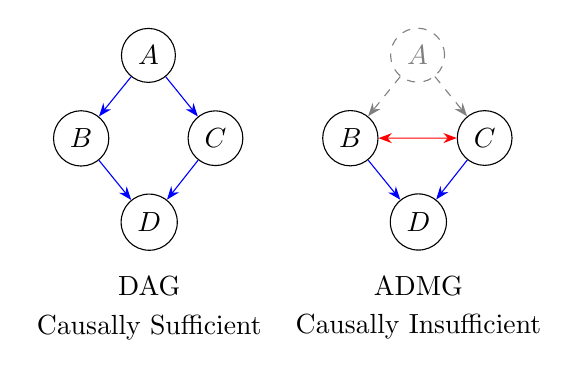
\begin{tikzpicture}[node distance=5mm]
                    \uncover<2-6>{
                    \node[draw, circle] (a) {\(A\)};
                    \node[draw, circle, below left=of a, yshift=-2mm] (b) {\(B\)};
                    \node[draw, circle, below right=of a, yshift=-2mm] (c) {\(C\)};
                    \node[draw, circle, below right=of b, yshift=-2mm] (d) {\(D\)};
                    \draw[-{Stealth}, blue] (a) -- (b);
                    \draw[-{Stealth}, blue] (a) -- (c);
                    \draw[-{Stealth}, blue] (b) -- (d);
                    \draw[-{Stealth}, blue] (c) -- (d);
                    \node[below=of d, yshift=3mm] (e) {DAG};
                    \node[below=of e, yshift=5mm] (f) {Causally Sufficient};
                }
                \uncover<3-6>{
                    \node[draw, circle, right=of c, xshift=5mm] (b1) {\(B\)};
                    \node[draw, circle, above right=of b1, yshift=2mm, gray, dashed] (a1) {\(A\)};
                    \node[draw, circle, below right=of a1, yshift=-2mm] (c1) {\(C\)};
                    \node[draw, circle, below right=of b1, yshift=-2mm] (d1) {\(D\)};
                    \draw[-{Stealth}, blue, color=gray, dashed] (a1) -- (b1);
                    \draw[-{Stealth}, blue, color=gray, dashed] (a1) -- (c1);
                    \draw[-{Stealth}, blue] (b1) -- (d1);
                    \draw[-{Stealth}, blue] (c1) -- (d1);
                    \draw[<->, >={Stealth}, red] (b1) -- (c1);
                    \node[below=of d1, yshift=3mm] (e1) {ADMG};
                    \node[below=of e1, yshift=5mm] (f1) {Causally Insufficient};
                }
                \end{tikzpicture}
            \end{column}
            \uncover<4-6>{
            \begin{column}{0.40\textwidth}
                \begin{center}
                    \underline{\textbf{Linear Gaussian SCMs}}
                \end{center}
                \[\mathbf{V} = \mathbf{\Theta V + U}\]
                \[\mathbf{U} \sim \mathcal{N}(\mathbf{0}, \mathbf{\Omega})\]
                \(\mathbf{V}\): observable variables \\
                \(\mathbf{U}\): unobservable variables \\
                \(\mathbf{\Theta}\): structural coefficients matrix \\
                \(\mathbf{\Omega}\): error covariances matrix \\
            \end{column}
        }
        \end{columns}
        \uncover<5-6>{
        In the presence of latent confounding, off-diagonal elements of \(\mathbf{\Omega}\) are non-zero.
    }
    \uncover<6>{
        \begin{definition}[Causal effect --- real world definition]
            A variable \(X\) has a causal effect on the variable \(Y\) if forcing \(X\) to take some value \(x_0\), the distribution of \(Y\)  explicitly depends on \(x_0\):
            \[\exists \,\, x_0 \in \mathcal{X} : P(Y|\textnormal{do}(X=x_0)) \neq P(Y)\]
        \end{definition}
    }
    \end{frame}

    \begin{frame}{Graph Classes and Problem Statement}
        \begin{columns}[T, onlytextwidth]
            \begin{column}{0.49\textwidth}
                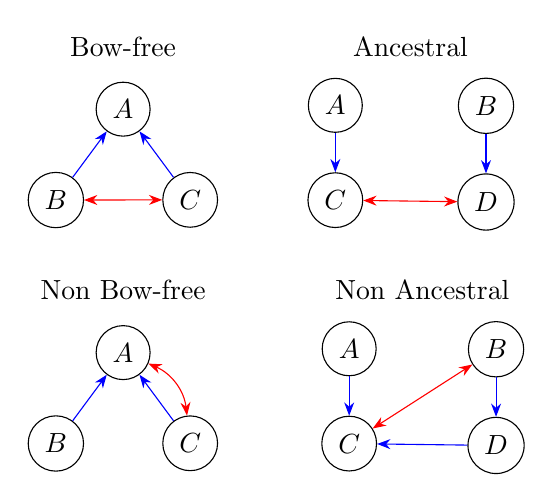
\begin{tikzpicture}[node distance=5mm]
                    % Bow-free
                    \uncover<1-4>{
                    \node[] (bf) {Bow-free};
                    \node[draw, circle, below=of bf, yshift=3mm] (a) {\(A\)};
                    \node[draw, circle, below left=of a, yshift=-3mm] (b) {\(B\)};
                    \node[draw, circle, below right=of a, yshift=-3mm] (c) {\(C\)};
                    \draw[->, >={Stealth}, blue] (b) -- (a);
                    \draw[->, >={Stealth}, blue] (c) -- (a);
                    \draw[<->, >={Stealth}, red] (b) -- (c);
                    % Non bow-free
                    \node[below=of a, yshift=-12mm] (nbf) {Non Bow-free};
                    \node[draw, circle, below=of nbf, yshift=3mm] (a1) {\(A\)};
                    \node[draw, circle, below left=of a1, yshift=-3mm] (b1) {\(B\)};
                    \node[draw, circle, below right=of a1, yshift=-3mm] (c1) {\(C\)};
                    \draw[->, >={Stealth}, blue] (b1) -- (a1);
                    \draw[->, >={Stealth}, blue] (c1) -- (a1);
                    \draw[<->, >={Stealth}, red] (c1) to[bend right] (a1);
                }
                \uncover<2-4>{
                    % Ancestral
                    \node[right=of bf, xshift=15mm] (an) {Ancestral};
                    \node[draw, circle, below left=of an, xshift=5mm, yshift=1mm] (a2) {\(A\)};
                    \node[draw, circle, below right=of an, xshift=-5mm, yshift=1mm] (b2) {\(B\)};
                    \node[draw, circle, below=of a2] (c2) {\(C\)};
                    \node[draw, circle, below=of b2] (d2) {\(D\)};
                    \draw[->, >={Stealth}, blue] (a2) -- (c2);
                    \draw[->, >={Stealth}, blue] (b2) -- (d2);
                    \draw[<->, >={Stealth}, red] (c2) -- (d2);
                    % Non Ancestral
                    \node[right=of nbf, xshift=9mm] (nan) {Non Ancestral};
                    \node[draw, circle, below left=of nan, xshift=9mm, yshift=1mm] (a3) {\(A\)};
                    \node[draw, circle, below right=of nan, xshift=-9mm, yshift=1mm] (b3) {\(B\)};
                    \node[draw, circle, below=of a3] (c3) {\(C\)};
                    \node[draw, circle, below=of b3] (d3) {\(D\)};
                    \draw[->, >={Stealth}, blue] (a3) -- (c3);
                    \draw[->, >={Stealth}, blue] (b3) -- (d3);
                    \draw[->, >={Stealth}, blue] (d3) -- (c3);
                    \draw[<->, >={Stealth}, red] (c3) -- (b3);
                }
                \end{tikzpicture}
            \end{column}
            \uncover<3-4>{
            \begin{column}{0.49\textwidth}
                \textbf{Bow-free ADMGs}
                \begin{enumerate}
                    \item In the case of Linear Gaussian SCMs are almost-everywhere identifiable, in the limit of infinite data
                    \item Can capture Verma Constraints
                \end{enumerate}
                \vspace{\baselineskip}
                \textbf{Ancestral ADMGs}
                \begin{enumerate}
                    \item In the case of Linear Gaussian SCMs are globally identifiable, in the limit of infinte data
                    \item Can't capture Verma Constraints
                    \item Are a subset of Bow-free ADMGs
                \end{enumerate}
            \end{column}
        }
        \end{columns}
        \uncover<4>{
        \begin{block}{Problem Statement}
            Causal Discovery on observational data for Linear Gaussian Structural Causal Models (SCMs), targeting ancestral and bow-free Acyclic Directed Mixed Graphs (ADMGs).
        \end{block}
    }
    \end{frame}

    \begin{frame}{Methodology}
        \begin{center}
            \begin{tikzpicture}
                \uncover<3-8>{
                \node[draw, inner sep=0] (optim) {
                    \begin{tikzpicture}[scale=1]
                        \clip (-1,-1) rectangle (1,1);
                        \draw[step=0.25, gray!30, very thin] (-1,-1) grid (1,1);
                        \draw[gray!50, thin] (-1,0) -- (1,0);
                        \draw[gray!50, thin] (0,-1) -- (0,1);
                        \draw[red] plot [smooth, tension=0.7] coordinates {
                            (-0.8, 0.8)
                            (-0.2, 0.5)
                            (0.6, 0.6)
                            (0.3, -0.2)
                            (-0.5, -0.4)
                            (0.2, -0.7)
                            (0.7, -0.5)
                        };
                        \fill[red!70] (0.7, -0.5) circle (1pt);
                    \end{tikzpicture}
                };
                \node[below=of optim, yshift=10mm] (label1) {CMA-ES, PPO};
                \node[above=of optim, yshift=-10mm] (label2) {search high dim space};
            }
            \uncover<4-8>{
                \node[draw, inner sep=0, right=of optim, xshift=20mm] (samples) {
                    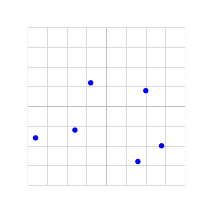
\begin{tikzpicture}[scale=1]
                        \clip (-1,-1) rectangle (1,1);
                        \draw[step=0.25, gray!30, very thin] (-1,-1) grid (1,1);
                        \draw[gray!50, thin] (-1,0) -- (1,0);
                        \draw[gray!50, thin] (0,-1) -- (0,1);
                        \fill[blue] (0.7, -0.5) circle (1.0pt);
                        \fill[blue] (-0.2, 0.3) circle (1.0pt);
                        \fill[blue] (0.4, -0.7) circle (1.0pt);
                        \fill[blue] (-0.9, -0.4) circle (1.0pt);
                        \fill[blue] (-0.4, -0.3) circle (1.0pt);
                        \fill[blue] (0.5, 0.2) circle (1.0pt);
                    \end{tikzpicture}
                };
                \node[above=of samples, yshift=-10mm] (label3) {\(z \in \mathbb{R}^{d^2}\)};
                \draw[->, >={Stealth}, teal!70, thick] (optim) to node [black, auto, swap] {sample points} (samples);
            }
            \uncover<5-8>{
                \node[below=of samples, yshift=-15mm] (sd) {Space of ADMGs};
                \draw[->, >={Stealth}, teal!70, thick] (samples) to node [black, auto] {\(\Phi_d(z)\)} (sd);
            }
            \uncover<6-8>{
                \node[below=of optim, yshift=-15mm] (bic) {BIC};
                \draw[->, >={Stealth}, teal!70, thick] (sd) to node [black, auto, swap] {RICF + data} (bic);
            }
            \uncover<7-8>{
                \draw[->, >={Stealth}, teal!70, thick] (bic) to node [black, auto] {update} node [black, auto, swap] {params} (label1);
            }
                \uncover<1-8>{
                \node[fit=(optim) (label1) (label2) (samples) (label3) (sd) (bic),draw, violet] (enclose) {};
                \node[above=of enclose, yshift=-10mm] (algo) {\textsc{Cadilac Algorithm}};
            }
                \uncover<2-8>{
                \node[above left=of optim, xshift=-1mm, yshift=1mm] (label4) {data, \(\mathcal{G}\)};
                \draw[->, >={Stealth}, teal!70, thick, double] (label4) to (enclose);
            }
            \uncover<8>{
                \node[below right=of sd, xshift=-8mm, yshift=3mm] (label5) {ADMG, PAG};
                \draw[->, >={Stealth}, teal!70, thick, double] (enclose) to (label5);
            }
            \end{tikzpicture}
        \end{center}
    \end{frame}

    \begin{frame}{Vec2ADMG Mappings}
        \vspace{-1em}
        \begin{columns}[T, onlytextwidth]
            \begin{column}{0.56\textwidth}
                \begin{definition}
                    \label{vec2admg}
                    \(\forall \,\, d \in \mathbb{N}^{+} \textnormal{ and } z \in \mathbb{R}^{d^2}\), \(p \in \mathbb{R}^d\) is the vector formed from the first \(d\) elements of \(z\), \(E_{\rightarrow}, E_{\leftrightarrow} \in \mathbb{R}^{d \times d}\) are strictly lower triangular matrices formed from the next \(\frac{d(d-1)}{2}\) and final \(\frac{d(d-1)}{2}\) elements of \(z\), respectively:
                    \begin{align*}
                        \Phi_{d}^{BF}(z)[D] &:= H\left(E_{\rightarrow} + E_{\rightarrow}^\top\right) \odot H\left(\textnormal{grad}(p)\right) \\
                        \Phi_d^{BF}(z)[B] &:= H\left(E_{\leftrightarrow} + E_{\leftrightarrow}^\top\right) \odot \Psi(D) \\
                        \Phi_d^{AN}(z)[D] &:= H\left(E_{\rightarrow} + E_{\rightarrow}^\top\right) \odot H\left(\textnormal{grad}(p)\right) \\
                        \Phi_d^{AN}(z)[B] &:= H\left(E_{\leftrightarrow} + E_{\leftrightarrow}^{\top}\right) \odot \Psi(D^+)
                    \end{align*}
                    where \(\Psi(M) := (I-M)\odot(I-M^\top)\), \(H(x) := 
                    \begin{cases}
                        1, & \textnormal{if } x > 0 \\
                        0, & \textnormal{if } x \leq 0
                    \end{cases}
                    \) is the Heaviside step function, \(\odot\) is the element-wise product, \(\textnormal{grad}(u)_{ij} := u_j - u_i\), and \(A^+\) is the transitive closure of \(A\).
                \end{definition}
            \end{column}
            \pause
            \hfill
            \begin{column}{0.40\textwidth}
                \vspace{\baselineskip}
                \textbf{Properties}
                \begin{enumerate}
                    \item One-step mappings
                        \pause
                    \item Unconstrained parameterisation of the space of ADMGs
                        \pause
                    \item \(\Phi_d^{BF}\) has time complexity \(\mathcal{O}(d^2)\)
                    \item \(\Phi_d^{AN}\) has time complexity \(\mathcal{O}(d^{2.8})\)
                        \pause
                    \item Automatic acyclicity
                    \item No differentiable constraints needed
                        \pause
                    \item Surjective
                        \pause
                    \item Scale and Translation Invariance
                \end{enumerate}
            \end{column}
        \end{columns}
    \end{frame}

    \begin{frame}{Optimization Algorithms}
        \begin{columns}[T, onlytextwidth]
            \begin{column}{0.49\textwidth}
                \textbf{PPO}
                \pause
                \begin{enumerate}
                    \item Deep RL algorithm
                    \item Stochastic Gradient Descent based optimizer
                        \pause
                    \item Tries to find optimal policy \(\pi_{\theta}\) which maximises \(J(\pi_{\theta}) = \mathbb{E}_{\tau \sim \pi_{\theta}}[\sum_{t=0}^{\infty}\gamma^{t}r_t]\)
                    \item Policy updates are limited to trust region to add stability to training
                        \pause
                    \item \(\pi_{\theta}(z) = \mathcal{N}(z;\mu_{\theta}, \textnormal{diag}(\sigma_{\theta}^2))\)
                        \pause
                    \item \(R(z) = -\frac{1}{n}\textnormal{BIC}(X, \Phi_d(z))\)
                        \pause
                    \item We do entropy annealing to help escape local minima
                        \pause
                    \item One-step environment - every \(z\) gives a graph
                        \pause
                    \item Designed to function well in high dimensional spaces
                        \pause
                    \item On-policy algorithm, sample in-efficient
                \end{enumerate}
            \end{column}
            \begin{column}{0.49\textwidth}
                \textbf{CMA-ES}
                \pause
                \begin{enumerate}
                    \item Evolutionary algorithm
                    \item Stochastic derivative-free black-box optimizer
                        \pause
                    \item Iterative algorithm: sample, rank, update loop
                        \pause
                    % \item Tries to find samples from the search space that maximise an objective function
                        % \pause
                    \item We restrict covariance matrix to be diagonal for scalability
                        \pause
                    \item Objective fn 
                        \(f_d(z) = \textnormal{BIC}\left(X, \Phi_d(z)\right) - \gamma \Gamma(z)\)
                        \(\Gamma(z) = \sum_{i < j}^{\{i, j\} < d} \min(|z_i - z_j|, \delta) + \sum_{k, k \geq d} \min(|z_k|, \delta)\)
                        \pause
                    \item Designed to function even in non-convex or ill-behaved landscapes
                        \pause
                    \item Sample efficient
                \end{enumerate}
            \end{column}
        \end{columns}
    \end{frame}

    \begin{frame}{Comparison Algorithms and Data Generation}
        \begin{columns}[T, onlytextwidth]
            \begin{column}{0.49\textwidth}
                \textbf{GFCI}
                \pause
                \begin{enumerate}
                    \item Hybrid Algorithm: Has constraint based and score based phases
                        \pause
                    \item Only outputs a PAG.
                        \pause
                    \item Used as a baseline for comparison.
                        \pause
                \end{enumerate}
                \vspace{\baselineskip}
                \textbf{DCD}
                \pause
                \begin{enumerate}
                    \item Differentiable constraints for acyclicity and to restrict search to bow-free/arid/ancestral graph classes
                        \pause
                    \item Uses modified RICF algorithm
                        \pause
                    \item Uses augmented Lagrangian to obtain unconstrained optimization problem
                        \pause
                    \item Solves the optimization problem with dual descent
                        \pause
                \end{enumerate}
            \end{column}
            \begin{column}{0.49\textwidth}
                \textbf{Synthetic Data Generation}
                        \pause
                \begin{enumerate}
                    \item Uses modified version of Erd\H{o}s-R\'{e}nyi random graph generation model
                        \pause
                    \item Modification accounts for existence of bidirected edges, requirement for bow-free/ancestral graphs
                        \pause
                    \item Inputs: average degree of graph skeleton \(\bar{\rho}\), fraction of directed edges \(f^{\rightarrow}\)
                        \pause
                    \item Guarantees: \(|\hat{E}| = \bar{\rho}d/{2} \pm 5\) and \(\widehat{f^{\rightarrow}} = f^{\rightarrow} \pm 0.1\)
                        \pause
                \end{enumerate}
                \begin{table}
                    \caption{\(\mathbf{\Theta}\) is the structural coefficients matrix and \(\mathbf{\Omega}\) error covariances matrix}
                    \begin{tabular}{l | l}
                        \hline
                        \textbf{Matrix} & \textbf{Distribution} \\ \hline
                        \(\mathbf{\Theta}\) & \(\mathcal{U}(\pm[0.5, 2])\) \\
                        Off-diag \(\mathbf{\Omega}\) & \(\mathcal{U}(\pm[0.4, 0.7])\) \\
                        Diag \(\mathbf{\Omega}\) & \(\mathcal{U}([0.7, 1.2] + \sum(|\mathbf{\Omega}_{i,-i}|)\) \\
                        \hline
                    \end{tabular}
                \end{table}
            \end{column}
        \end{columns}
    \end{frame}
    
    \begin{frame}{Sachs Dataset}
        \uncover<1-3>{
        \begin{table}
            \centering
            \begin{threeparttable}[b]
                \caption{Performance of Algorithms on Sachs Dataset \label{sachs_table}}
                \begin{tabular}{l | c | c | c | c}
                    \hline
                    & \textbf{SHD} (\(\downarrow\)) & \(|E \cap \hat{E}| / |\hat{E}|\)\tnote{1} (\(\uparrow\)) & \textbf{PAG} \(\mathbf{F}_1\)\tnote{3} (\(\uparrow\)) & \(\tau\)\tnote{2} (\(\downarrow\)) \\ \hline
                    \textbf{DCD} & 53 & 3 / 43 & 0.47 & 249.5 \\
                    \textbf{CMA-ES} & 22 & 1 / 8& 0.58 & 105.7 \\
                    \textbf{Relcadilac} & 23 & 1 / 9 & 0.48 & 1029.2 \\
                    \hline
                \end{tabular}
                \begin{tablenotes}
                    \item [1] \(|E \cap \hat{E}|\) is the number of correct predicted edges, and \(|\hat{E}|\) is the total number of predicted edges.
                    \item [2] \(\tau\) is the runtime of the algorithm in seconds.
                    \item [3] The \(F_1\) score is computed on the skeleton of the PAG.
                \end{tablenotes}
            \end{threeparttable}
        \end{table}
    }
        \vspace{\baselineskip}
        \begin{tikzpicture}[node distance=5mm]
            \uncover<2-3>{
            \node[] (pip3) {PIP3};
            \node[right=of pip3] (plcg) {PLC\(_\gamma\)};
            \node[above right=of plcg] (pip2) {PIP2};
            \node[right=of pip2] (pkc) {PKC};
            \node[above right=of pkc] (raf) {Raf};
            \node[below right=of raf] (mek) {Mek};
            \node[below right=of mek] (erk) {Erk};
            \node[below=of raf] (p38) {p38};
            \node[below=of p38] (jnk) {JNK};
            \node[below=of jnk] (akt) {Akt};
            \node[below=of pkc] (pka) {PKA};
            \draw[->, >={Stealth}, teal] (pip3) -- (plcg);
            \draw[->, >={Stealth}, teal] (pip3) -- (akt);
            \draw[<->, >={Stealth}, teal] (pip3) -- (pip2);
            \draw[->, >={Stealth}, teal] (plcg) -- (pip2);
            \draw[->, >={Stealth}, teal] (plcg) -- (pkc);
            \draw[->, >={Stealth}, teal] (pip2) -- (pkc);
            \draw[->, >={Stealth}, teal] (pkc) -- (raf);
            \draw[->, >={Stealth}, teal] (pkc) -- (p38);
            \draw[->, >={Stealth}, teal] (pkc) -- (jnk);
            \draw[->, >={Stealth}, teal] (pka) -- (raf);
            \draw[->, >={Stealth}, teal] (pka) -- (p38);
            \draw[->, >={Stealth}, teal] (pka) -- (jnk);
            \draw[->, >={Stealth}, teal] (pka) -- (erk);
            \draw[->, >={Stealth}, teal] (pka) -- (akt);
            \draw[->, >={Stealth}, teal] (raf) -- (mek);
            \draw[->, >={Stealth}, teal] (mek) -- (erk);
            \node[above=of label1] (label3) {};
            \node[above=of label2] (label4) {};
            \node[right=of label4, xshift=-5mm] (title2) {True};
            \draw[>={Stealth}, teal, thick] (label3) -- (label4);
        }
            % CMA-ES
        \uncover<3>{
            \draw[->, >={Stealth}, red] (pip3) to[bend left] (plcg);
            \draw[->, >={Stealth}, red] (pip3) to[bend left] (pip2);
            \draw[->, >={Stealth}, red] (akt) to[bend left] (erk);
            \draw[->, >={Stealth}, red] (akt) to[bend left] (pka);
            \draw[->, >={Stealth}, red] (erk) to[bend left] (pka);
            \draw[->, >={Stealth}, red] (jnk) to[bend left] (pkc);
            \draw[<->, >={Stealth}, red] (pkc) to[bend left] (p38);
            \node[right=of erk] (label1) {};
            \node[right=of label1] (label2) {};
            \node[right=of label2, xshift=-5mm] (title1) {CMA-ES};
            \draw[>={Stealth}, red, thick] (label1) -- (label2);
        }
        \end{tikzpicture}
    \end{frame}

    \begin{frame}{Performance Plots I}
        \textbf{Varying Parameters}: 
        Sample Size, 
        Number of Nodes, 
        Average Degree of Skeleton, 
        Fraction of Directed Edges \\
        \textbf{Metrics Captured}: 
        Structural Hamming Distance (lower is better), 
        \(F_1\) score of the edges of the PAG Skeleton (higher is better),
        Fractional Excess BIC score (lower is better)
        \includegraphics[width=\textwidth]{/mnt/windows/Users/lordh/Documents/LibraryOfBabel/Projects/thesis/diagrams/to_include_in_paper/pag_skeleton_f1_shd_nodes_samples.pdf}
    \end{frame}

    \begin{frame}{Performance Plots II}
        \includegraphics[width=\textwidth]{/mnt/windows/Users/lordh/Documents/LibraryOfBabel/Projects/thesis/diagrams/to_include_in_paper/varying_frac_dir_deg_thresh_pag_skeleton_f1.pdf} \\
        \pause
        \includegraphics[width=\textwidth]{/mnt/windows/Users/lordh/Documents/LibraryOfBabel/Projects/thesis/diagrams/to_include_in_paper/varying_frac_dir_deg_thresh_pred_bic_excess.pdf}
    \end{frame}

    \begin{frame}{Conclusion and Future Work}
        \textbf{Conclusion}
        \begin{enumerate}
            \item modular framework for Causal Discovery under unmeasured confounding
                \pause
            \item converts a combinatorial discrete optimization problem into a continuous optimization approach
                \pause
            \item novel Vec2ADMG mappings for Bow-free and Ancestral ADMGs
                \pause
            \item Evaluates use of CMA-ES and PPO as stochastic optimizers
                \pause
            \item PPO suffers from long runtimes and sample in-efficiency
                \pause
            \item CMA-ES emerges as superior approach, being faster than the DCD algorithm while matching or surpassing its results
                \pause
        \end{enumerate}

        \vspace{\baselineskip}
        \textbf{Future Work}
        \pause
        \begin{enumerate}
            \item Explore the SAC RL algorithm for potentially better sample efficiency than PPO
                \pause
            \item RICF algorithm bi-directed connected components-based decomposition and caching for potential speedup in sparse graphs
                \pause
            \item Extend the Vec2ADMG mappings to include other graph classes like arid graphs
        \end{enumerate}
    \end{frame}
    \begin{frame}{Key References}
        \begin{enumerate}
            \item B. Duong, H. Le, B. Huang, and T. Nguyen, "Reinforcement learning for causal discovery without acyclicity constraints," Transactions on Machine Learning Research, 2025. [Online]. Available: https: //openreview.net/forum?id=sNzBi8rZTy

            \item  R.  Bhattacharya, T.  Nagarajan, D.  Malinsky, and I.  Shpitser, "Differentiable causal discovery under unmeasured confounding," in Proceedings of The 24th International Conference on Artificial Intelligence and Statistics, ser. Proceedings of Machine Learning Research, A. Banerjee and K. Fukumizu, Eds., vol. 130.  PMLR, Apr 2021, pp. 2314–2322. [Online]. Available: https://proceedings.mlr.  press/v130/bhattacharya21a.html
        \end{enumerate}
    \end{frame}
\end{document}
